%
% main.tex -- Paper zum Thema fpga
%
% (c) 2019 Hochschule Rapperswil
%
\chapter{FPGA Implementation der schnellen Wavelet-Transformation\label{chapter:fpga}}
\lhead{FPGA Implementation der schnellen Wavelet-Transformation}
\begin{refsection}
\chapterauthor{Jonas Gründler und Nicolas Tobler}

\section{Introduction}
\rhead{Introduction}
In this paper we study the implementation of a discrete Wavelet Transform and inverse transforming using VHDL.
But why VHDL? VHDL is a language for programming hardware and we wanted to implement the Wavelet Transformation in hardware.
This beacause first, we wanted to use some of the knowledge obtained in this course and second beacause we wanted to see if it is possible for us to implement this transformation in hardware.
Implementing the Wavelet Transformation in hardware has some significant benefits.
First of all speed. Implementations of arithmetic operations in hardware are much faster than in software.
If you further use your VHDL-Code on a FPGA you can parallelize as much of this operations as possible, which is another speed boost. 
Secondly, if well implemented and because of the speed, you can run your transformation nearly in real time.
If you try to transform and modify audio signals, which are sampled with 44 kHz you get, because of the clock speed of the FPGA, which is about 100 MHz, over 1000 arithmetic operations for every audio sample.
In the next few pages we guide through the theory used, some design considerations and at last through our steps of developing a basic but functional Wavelet Transformation in VHDL. 

\section{Lifting Scheme}
\rhead{Lifting Scheme}

The Transformation algorithm used is adopted from a paper of Ingrid Daubechies and Wim Sveldens \cite{fpga:Daubechies1998} and called Lifting. 
The Lifting Scheme is an widely used algorythm which is two times more efficient in termes of multiplication uses than normal Wavelet Transformations.
The Lifting Scheme factorizes any discrete Wavelet Transform  with finite filters into a series of elementary covolutions (Lifting Steps).
This reduces the number of arithmetic operations nearly by a factor of two.
This decomposition is equivalent to a factorisation of the polyphase matrix of the wavelet filter into elementary matrices. 
To describe the underlying wavelet Filters the z-transform notation is used.
The z-transform of a FIR (finite impulse response) filter \textit{\textbf{h}} is a laurent polynomial given by
\begin{equation}\label{equ:impulse}
	H(z) = \sum h_k z^{-k}
\end{equation}

%https://en.wikipedia.org/wiki/Lifting_scheme
%http://wavelets.org/schemes-lifting.php

\subsection{Polyphase Decomposition \label{fpga:polyphase}}

In our case we subsample the input signal by a factor of two.
This corresponds to splitting the signal into two sub channels (even and odd samples).
The polyphase decomposition is a algebraic way of describing the filter in matrices.
The polyphase components are the filter components of the sub channels. 
We can separate equation \ref{equ:impulse} into its even- and odd-indexed terms
\begin{equation}
	H(z) = \sum_{n=-\infty}^{\infty} h(2n)z^{-2n} + z^{-1} \sum_{n=-\infty}^{\infty} h(2n+1)z^{-2n}
\end{equation}
Following this scheme the polyphase components of the filter are defined as follows
\begin{equation}
E_0(z) = \sum_{n=-\infty}^{\infty} h(2n)z^{-n}
\end{equation}
\begin{equation}
E_1(z) = \sum_{n=-\infty}^{\infty} h(2n+1)z^{-n}
\end{equation}
which corresponds to the even and odd filter components.
Now $H(z)$ can be written in terms of the polyphase components
\begin{equation}
H(z)=E_{0}(z^2)+z^{-1} E_1(z^2)
\end{equation}
These coefficients are then placed in the so called Polyphase Matrix.
\begin{equation}
	P(z) = 
	\begin{bmatrix}
	h_e(z) & g_e(z) \\
	h_o(z) & g_o(z)
	\end{bmatrix}
\end{equation}

\begin{figure}
	\centering
	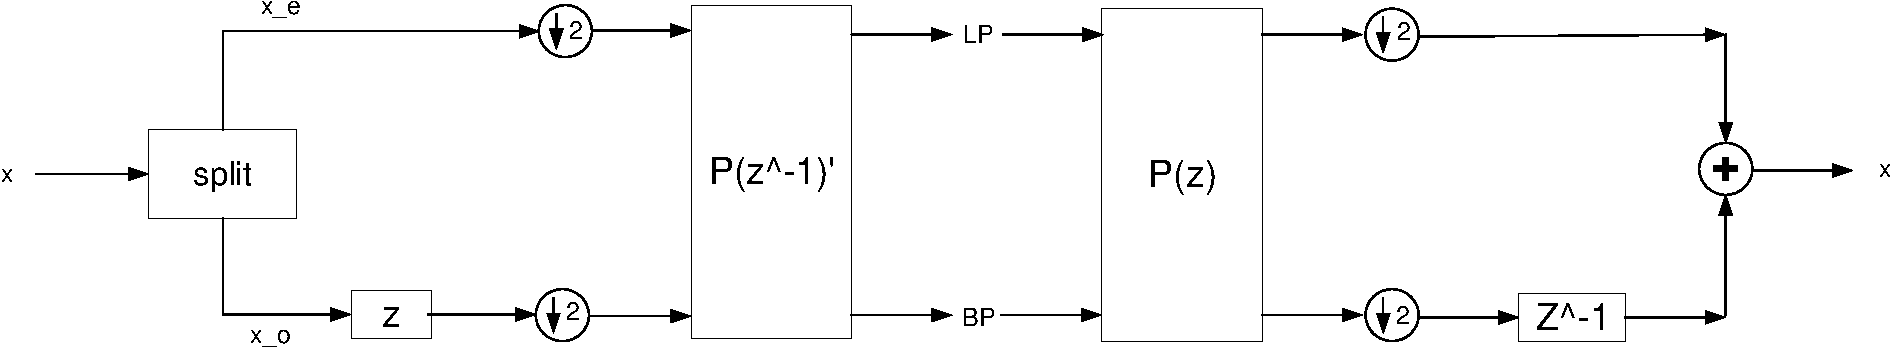
\includegraphics[width=\textwidth]{images/lifting_step_wavelet.pdf}
	\caption{Wavelet transformation with Lifiting Steps \label{fpga:lstp_wavelet}}
\end{figure}
Where $h_e(z)$ are the even- and $h_o(z)$ are the odd coefficients of the low pass filter.
$g(z)$ is the corresponding high pass filter. 
Because of its simplicity we first choose the Haar Wavelet.
In z notation $g(n)$ are the Father Wavelet coefficients whereas $h(n)$ are the corresponding Mother Wavelet coefficients. 
\begin{equation}
{\mathcal {Z}} \{h(n)\} = 1 + z^{-1}
\end{equation}
\begin{equation}
{\mathcal {Z}} \{g(n)\} = 1 - z^{-1}
\end{equation}
If we split these coefficients into even and odd components and fill them into the Polyphase Matrix we get 

\begin{equation*}
P(z) =
\begin{bmatrix}
1 & -\frac{1}{2} \\
1 & \frac{1}{2}
\end{bmatrix}
 = 
 \begin{bmatrix}
 1 & 0 \\
 1 & 1
 \end{bmatrix}
 \cdot
 \begin{bmatrix}
 1 & -\frac{1}{2} \\
 0 & 1
 \end{bmatrix}
\end{equation*}

The term on the right side is a possible factorization which results in lifting steps.
This factorizations produces diagonal matrices which are easy to compute and are the lifting steps.
This corresponds to the following implementation of the forward transform \cite{fpga:Daubechies1998}.
\begin{equation}
	\begin{aligned}
	s_l^{(0)} &= x_{2l} \\
	d_l^{(0)} &= x_{2l+1} \\ 
	d_l &= d_l^{(0)} - s_l^{(0)} \\
	s_l &= s_l^{(0)} + \frac{1}{2}d_l
	\end{aligned}
\end{equation}
where $x_{n}$ is the incoming sample stream.
The analysis side is in the following form:
\begin{equation*}
P(z^{-1})^ =
\begin{bmatrix}
\frac{1}{2} & \frac{1}{2} \\
-1 & 1
\end{bmatrix}
= 
\begin{bmatrix}
1 & \frac{1}{2} \\
0 & 1
\end{bmatrix}
\cdot
\begin{bmatrix}
1 & 0 \\
-1 & 1
\end{bmatrix}
\end{equation*}
In this case the inverse transformation is 
\begin{equation}
\begin{aligned}
s_l^{(0)} &= s_l - \frac{1}{2}d_l \\
d_l^{(0)} &= d_l + s_l \\ 
x_{2l+1}& =d_l^{(0)} \\
x_{2l} &= s_l^{(0)}
\end{aligned}
\end{equation}
and the original stream can be fully recovered.
In the next section we try to implement this algorithm in VHDL.

\section{Implementation}

\subsection{Design Considerations}

When implementing an algorithm in hardware, a lot of design considerations must be made in advance.
The hardware architecture is very dependent of the application.
A hardware block can be optimized for various points, such as high accuracy, low latency, high data rate, low area and low power consumption.
Since this work is not based on a defined objective, we must come up with our own design specifications.

In most cases, which do not require low latency and high data rates, a digital signal processor would be a better choice than a custom VHDL-implemented hardware.
A sequential processor unit is computationally very efficient, and requires almost no area compared to most VHDL solutions, however it features a significantly higher latency.
Hence, the implementation should feature low latency and high data rate as its main objectives in order to provide a VHDL solution, that is actually reasonable.
The application should make use of on of the biggest advantages of custom hardware which is parallelism.
Performing calculations in parallel leads to higher throughput, and allows data rates which are as fast as the clock speed of the logic.
The strengths of the aspired implementation are thus high speed and low latency processing suitable for real-time applications.

Two hardware blocks should be implemented for both forward wavelet and inverse wavelet transform.
The forward algorithm should have a 16-bit signed number as its input and outputs a given number of wavelet coefficients as a stream.
Th main priority is to implement the Haar wavelet.
A optional goal is the implementation of a higher order wavelet, such as the orthogonal Daubechies-4 wavlelet.


%The question is now, how do we implement the algorithm.
%There are a few possible ways to code algorithms in VHDL.
%As you can see in figure \ref{fpga:designcon} there are two major directions one can take.
%
%\begin{itemize}
%	\item \textbf{Slow} The slow approach is also the cheap way to go. In this case the power requirements are lower and also the used chip area is smaller. This results in slower computation and because of the smaller area the parallelization is also limited.
%	
%	\item \textbf{Fast} The fast approach is the expensive way to go. You use big, fast and because of this more powerhungry hardware. They need also a bigger area. The benefits are that you are able, beside from higher processing speed, to parallelize your algorithm. This allows you to process high data rates and do this, depending on the application, in realtime.  
%\end{itemize}
%The right way needs to be chosen according to the application. In our case we chose the fast and highly parallelized branch. This because our algorithm is comparably simple and can be parallelized even on smaller devices. 
%
%\b
%egin{figure}
%	\centering
%	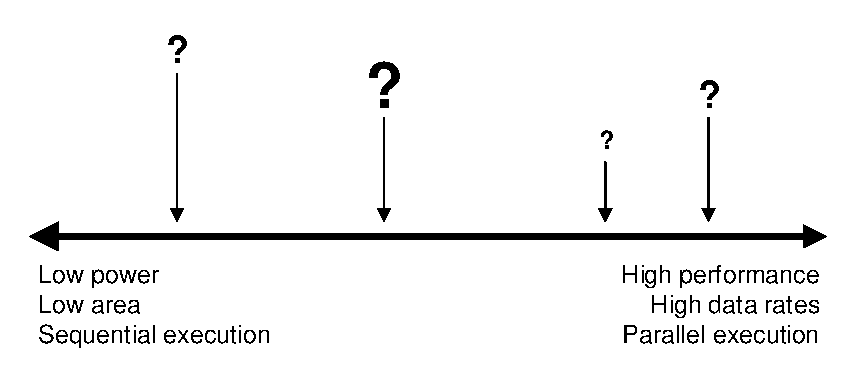
\includegraphics[width=0.8\textwidth]{images/design_considerations.pdf}
%	\caption{Design considerations \label{fpga:designcon}}
%\end{figure}

\subsection{Idea}


The mathematical description of the forward transform, as described in section ???, % provide reference to a formula
is noncausal and thus not implementable in a stream based fashion.
The noncausality is apparent from the positive z-exponent. %TODO z-exponent better word??


In order to make the forward transform implenetable, it has to be delayed to be fully causal again.


\subsection{Architecture}

The VHDL hardware consists of three main blocks, as depicted in figure \ref{fpga:fig:architecture.pdf}
The forward transform block contains multiple wavlet-blocks which together perform a multiresolution analysis.
Since each layer splits a input data stream in half, this block is called \texttt{braching}.
It takes a 16-bit number as its input which is processed when the associated ready signal is driven high.
If this ready signal is always driven high, the input value is sampled each clock cycle.
The outputs consist of an array of wavelet coefficients, each of 16 bits, which are accompanied with a vector of ready signals. 

\begin{figure}
	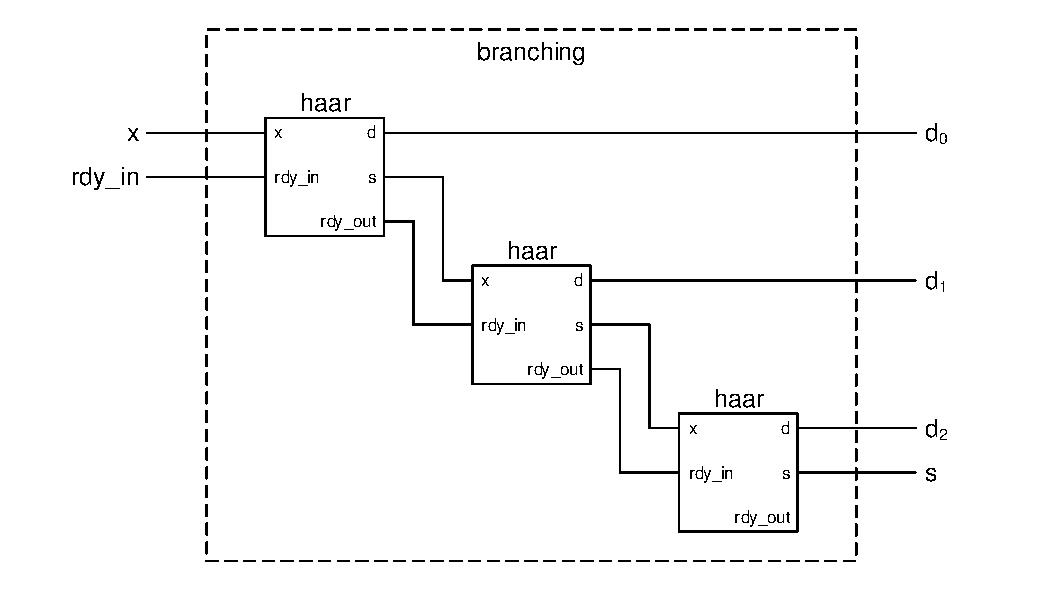
\includegraphics[width=0.49\textwidth]{images/branching.pdf}
	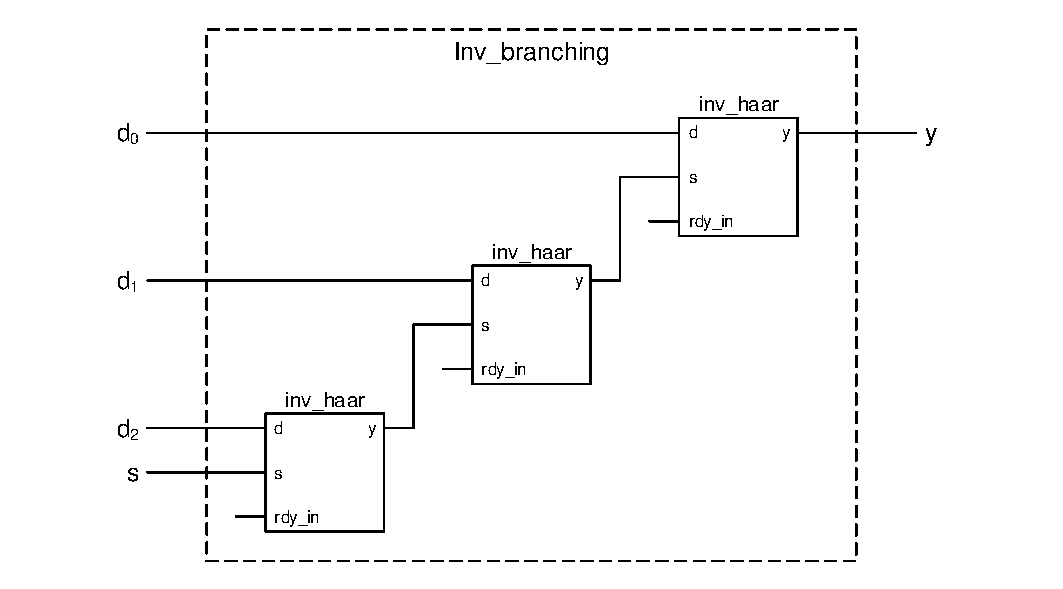
\includegraphics[width=0.49\textwidth]{images/inv_branching.pdf}
	\caption{Branching and inverse branching \label{fpga:fig:architecture}}
\end{figure}

The inverse wavelet transform has an analogous outline.
The input coefficients are reconstructed to a 16-bit signed output number in the \texttt{inv\_branching} block, which holds several blocks of inverse wavelet transforms.

Finally a third block is needed to delay the coefficients.
The wavelet transform is very expensive to calculate in one single clock cycle.
In order to provide low-latency regardless, a compromize has been made, which tolerates a delay of one cyle in each layer of the muliresolution analysis.

The coefficients except the one with the lowest frequency must be delayed for the inverse algorithm.

%TODO make figure of delay

\subsubsection{Branching}

The before mentioned transform is not very interesting. On the other hand, what would be challenging to implement is a recursive use of these blocks to get further coefficients of different frequencies.
We called this Branching. The Lowpass output ($s$) samples of a Haar block are connected to another Haar block which does another transformation to get more detail. Because of this we need the also delayed ready signal from the last block because these coefficients are changing with half of the speed now. 

The inverse branching  is then used to reconstruct the original signal from all the different transformations and coefficients.





\subsection{Testing}

The test structure contains the forward transform, followed by the inverse transform, which should recover the original signal from the processed coefficients.
The test setup is shown in figure \ref{fpga:fig:testing}
The output should resemble the input, delayed by the latency of the whole pipeline.

Vivado Toolchain from Xilix has been used to simulate the VHDL modules.
The wavelet transforms have also been implemented numerically identical in MATLAB in order to provide a direct comparison. 
A set of helper modules have been implemented in VHDL 2008, which are able to read and write test vectors and results from or to a file.
These modules provide an an easy way to inject test data from the MATLAB enviroment.
After the VHDL simulation finishes, the results are again fed into MATLAB for validation.




The idea is to have a data stream \texttt{x} an a ready \texttt{rdy} signal. The ready signal indicates when the input from the data stream is valid. The input is only read and processed if the ready signal is high. Then we build a block which contains the signal processing which was presented in section \ref{fpga:polyphase}. The Block then throws out the wavelet coefficients and also the ready signal for further processing. In a next stage a block for inverse transformation is used to recover the input signal.

\begin{figure}
	\centering
	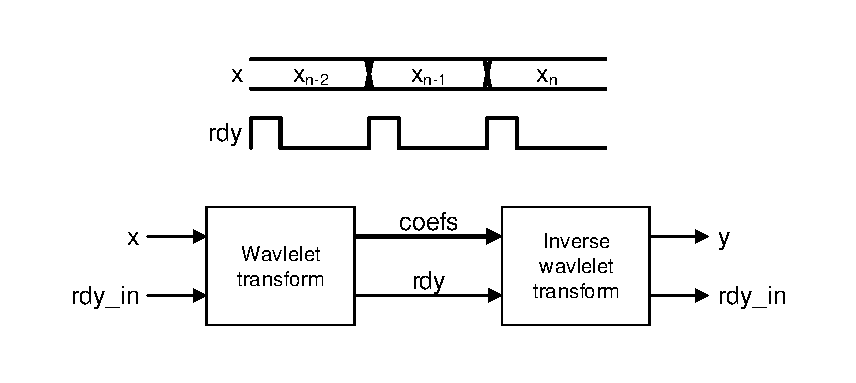
\includegraphics[width=0.8\textwidth]{images/idea.pdf}
	\caption{Basic idea and important building blocks \label{fpga:idea}}
\end{figure}
In this block we then implement the Wavelet Transformation with, in our case, the Haar Wavelet. Another goal was to create a structure to implement different wavelet transformations later. In this way of implementation  it should be possible to implement transformations with different wavelets in the same block (Picture \ref{fpga:haar_inv_haar}). 

\begin{figure}[h]
	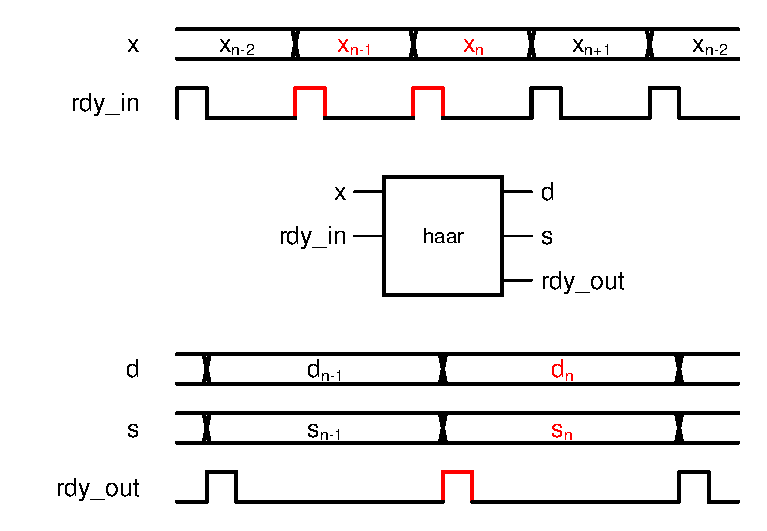
\includegraphics[width=0.49\textwidth]{images/haar.pdf}
	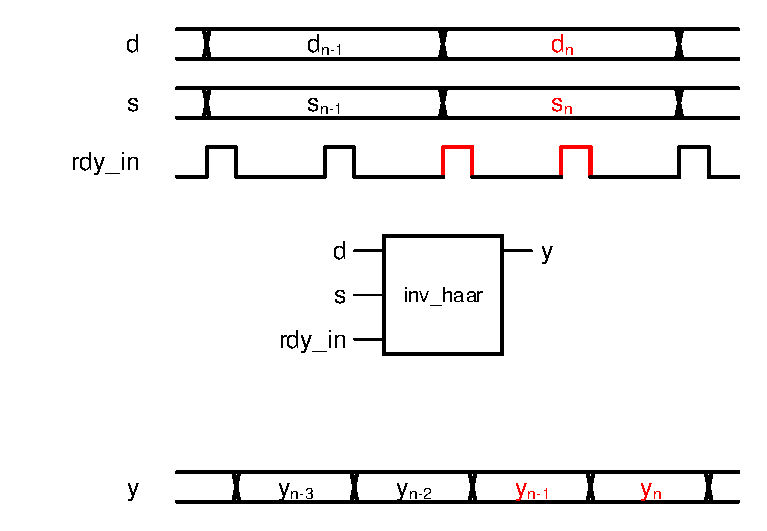
\includegraphics[width=0.49\textwidth]{images/inv_haar.pdf}
	\caption{Haar und inverse Haar transformation \label{fpga:haar_inv_haar}}
\end{figure}

%\begin{figure}[h!]
%	\centering
%	\begin{subfigure}[b]{\linewidth}
%		\centering
%		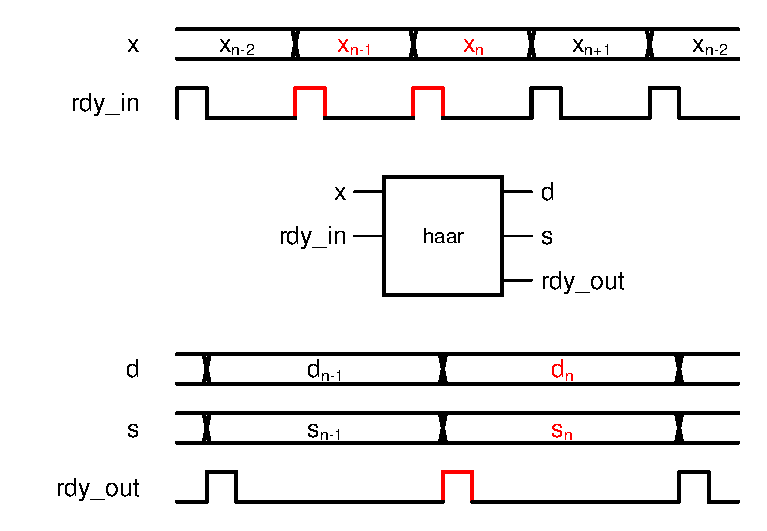
\includegraphics[width=0.49\textwidth]{images/haar.pdf}
%		\caption{Haar}
%	\end{subfigure}
%	\begin{subfigure}[b]{\linewidth}
%		\centering
%		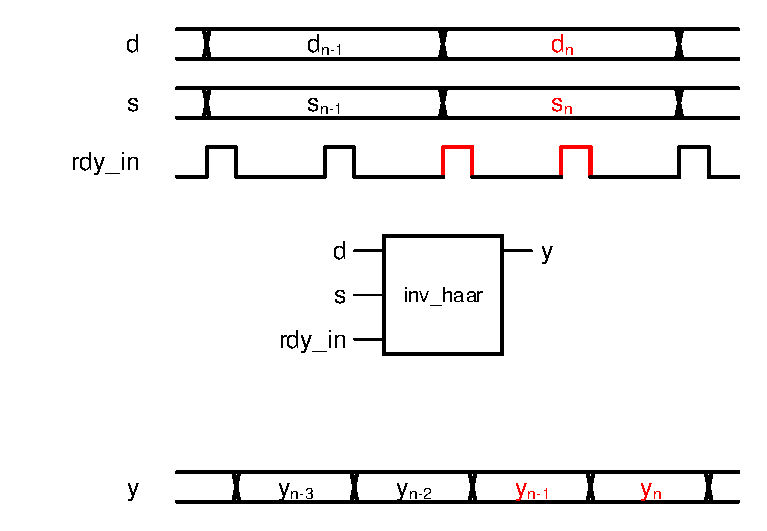
\includegraphics[width=0.49\textwidth]{images/inv_haar.pdf}
%		\caption{Inverse haar}
%	\end{subfigure}
%	\caption{Haar and inverse Haar transformation \label{fpga:haar_inv_haar}}
%\end{figure}

In this picture it is also visible that for every two input samples we get two wavelet coefficients. This corresponds to the sub sampling into two streams. The ready signal gets also delayed to match the speed of the output coefficients. In the inverse Haar block the coefficients get reconstructed to the original input stream.







\section{Conclusion}
\rhead{Conclusion}

\printbibliography[heading=subbibliography]
\end{refsection}
